\section{Lösungsansatz}

Zur Berechnung größerer Graphen gibt es sogenannten metaheuristische Verfahren die keine optimale Lösung garantieren.
Durch probabilistische Schätzungen und heuristische Verfahren können jedoch gute Lösungen gefunden werden.
\\\\
Eines dieser metaheuristischen Verfahren ist der Ant Algorithm (auch \glqq Ant Colony Optimization\grqq{} oder \glqq \acs{aco}\grqq{} genannt).
Dies ist ein Algorithmus der sich an dem Verhalten von Schwärmen von Tieren orientiert.
Ein Schwarm besteht aus einer Gruppe von \glqq Agenten\grqq{} die miteinander kommunizieren, um eine Lösung zu finden.
Der \acs{aco} basiert auf dem Verhalten von Ameisen, die Pfade zu Nahrungsquellen aufspüren.
\\
Der Algorithmus simuliert die Aktivitäten von Ameisen, die zufällig durch die Städte wandern und dabei Informationen über die Qualität der verschiedenen möglichen Pfade sammeln.
Bei jeder Bewegung einer Ameise werden auf dem gewählten Pfad Pheromone (Duftstoffe) hinterlassen.
Diese Informationen werden dann verwendet, um die Wahrscheinlichkeit zu bestimmen, dass eine bestimmte Ameise einen bestimmten Pfad wählt, wenn sie von einer Stadt zu einer anderen reist. 
\\
Zur weiteren Optimierung der Tour werden nacheinander mehrere Generationen von Schwärmen durchlaufen.
Jede Generation bekommt die Wahrscheinlichkeiten der Pfade der vorherigen Generation und baut darauf auf.
Auf diese Weise kann der Algorithmus schrittweise die optimale Tour durch die Städte bestimmen.

\begin{figure}[H]
    \centering
    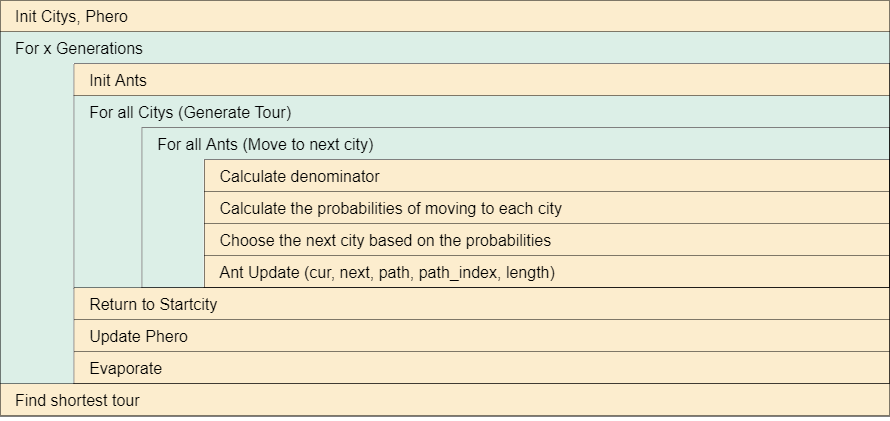
\includegraphics[width=16cm]{../images/struktog.png}
    \caption{Algorithmus Struktogramm}
    \label{fig:struktogramm}
\end{figure}

\section{Implementierung inklusive Schwierigkeiten}
1 - 2 Seiten\\
\subsection*{C Implementierung}

Damit die Verfahren vergleichbar sind, brauchen wir immer gleiche Ausgangsdaten und können diese daher nicht generieren, sondern laden diese über CSV Dateien.
Dabei besteht jede Stadt aus zwei Koordinaten, die in den Dateien gehalten werden.
Die Distanz, zur Vereinfachung die Luftlinie, zwischen zwei Städten wird mittels der Koordinaten berechnet.
\\\\
Alle Daten zur Berechnung des Pfades sind in einem Ameisen-Struct enthalten.
Dies umfasst unter anderem den Pfad der Ameise, welche Städte sie besucht hat und die Länge der Tour.
Jene Daten werden bei jeder Generation zurückgesetzt.
Im Gegensatz dazu wird die Pheromonmatrix nicht zurückgesetzt und lässt somit die Ergebnisse der vorherigen Generationen mit einfließen.
Nach jedem Durchlauf wird die Pheromonmatrix abhängig von den berechneten Tourlängen angepasst und eine natürliche Verdunstung durchgeführt.
\\\\
Abschließend wird aus der letzten Generation die beste Tour gefunden und ausgegeben.
\\\\
Zur Bewertung des Ergebnisses haben wir folgendes \href{https://poolik.github.io/visual-aco/}{ACO-Onlinetool} verwendet. 
\begin{table}[h]
    \centering
    \begin{tabular}{|l|l|}
    \hline
                    & Pfadlänge    \\ \hline
    Online ACO Tool & $\sim$13.000 \\ \hline
    Plain C         & $\sim$13.500 \\ \hline
    \end{tabular}
    \caption{\label{demo-table}Pfadlängenvalidierung}
\end{table}

\begin{figure}[H]
    \centering
    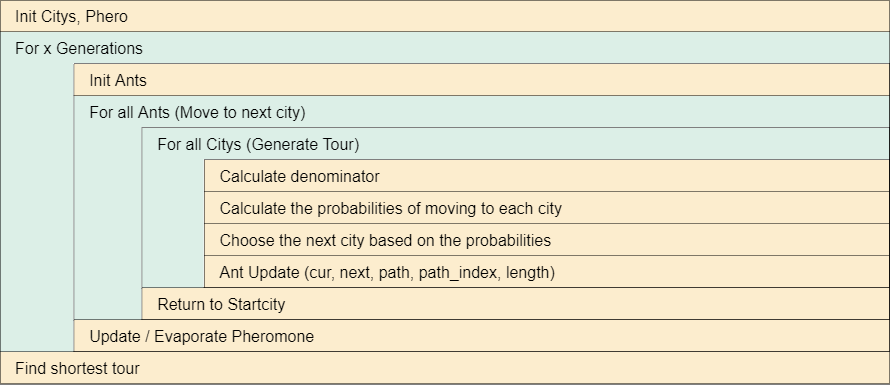
\includegraphics[width=16cm]{../images/struktog-optimiert.png}
    \caption{Algorithmus Struktogramm Optimiert}
    \label{fig:struktogramm-optimiert}
\end{figure}

\subsection*{OpenMP Optimierung}

\subsection*{OpenCL Optimierung}

\section{Bewertung}
Bewertung des Ansatzes und der performance-limitierenden Faktoren (1-2 Seiten)
